\chapter{Experiments in RGBD sensing using DepthAI} \label{experiments_oak_d}

\section{Overview}

In this chapter we explore the capabilities of the OAK-D camera using the DepthAI Viewer software to understand its functionalities. This exploration provided insights into the camera's real-time 3D reconstruction and its Vision Processing Unit (VPU) capabilities. Subsequently, we experimented with the Spectacular AI SDK to further test the camera's performance, especially in mapping and person detection scenarios.


\section{DepthAI Viewer}

To begin exploring the capabilities of the camera, I initiated my efforts by testing the example software provided by the camera's manufacturer, namely DepthAI Viewer\footnote{\url{https://github.com/luxonis/depthai-viewer}}. This software proved invaluable for its ability to showcase the camera's functionalities effectively.

Upon installation, I gained access to a user-friendly interface that allowed me to view images captured by the camera in real time. Additionally, the software facilitated real-time 3D reconstruction of the camera's surroundings, as depicted in Figure~\ref{fig:DAI_3d}. Notably, the DepthAI Viewer leveraged the Vision Processing Unit (VPU) embedded within the device, thereby enabling comprehensive exploration of its capabilities, as illustrated in the top left corner of Figure~\ref{fig:DAI_person_detection}.

\FloatBarrier
\begin{figure}[htbp]
	\centering
	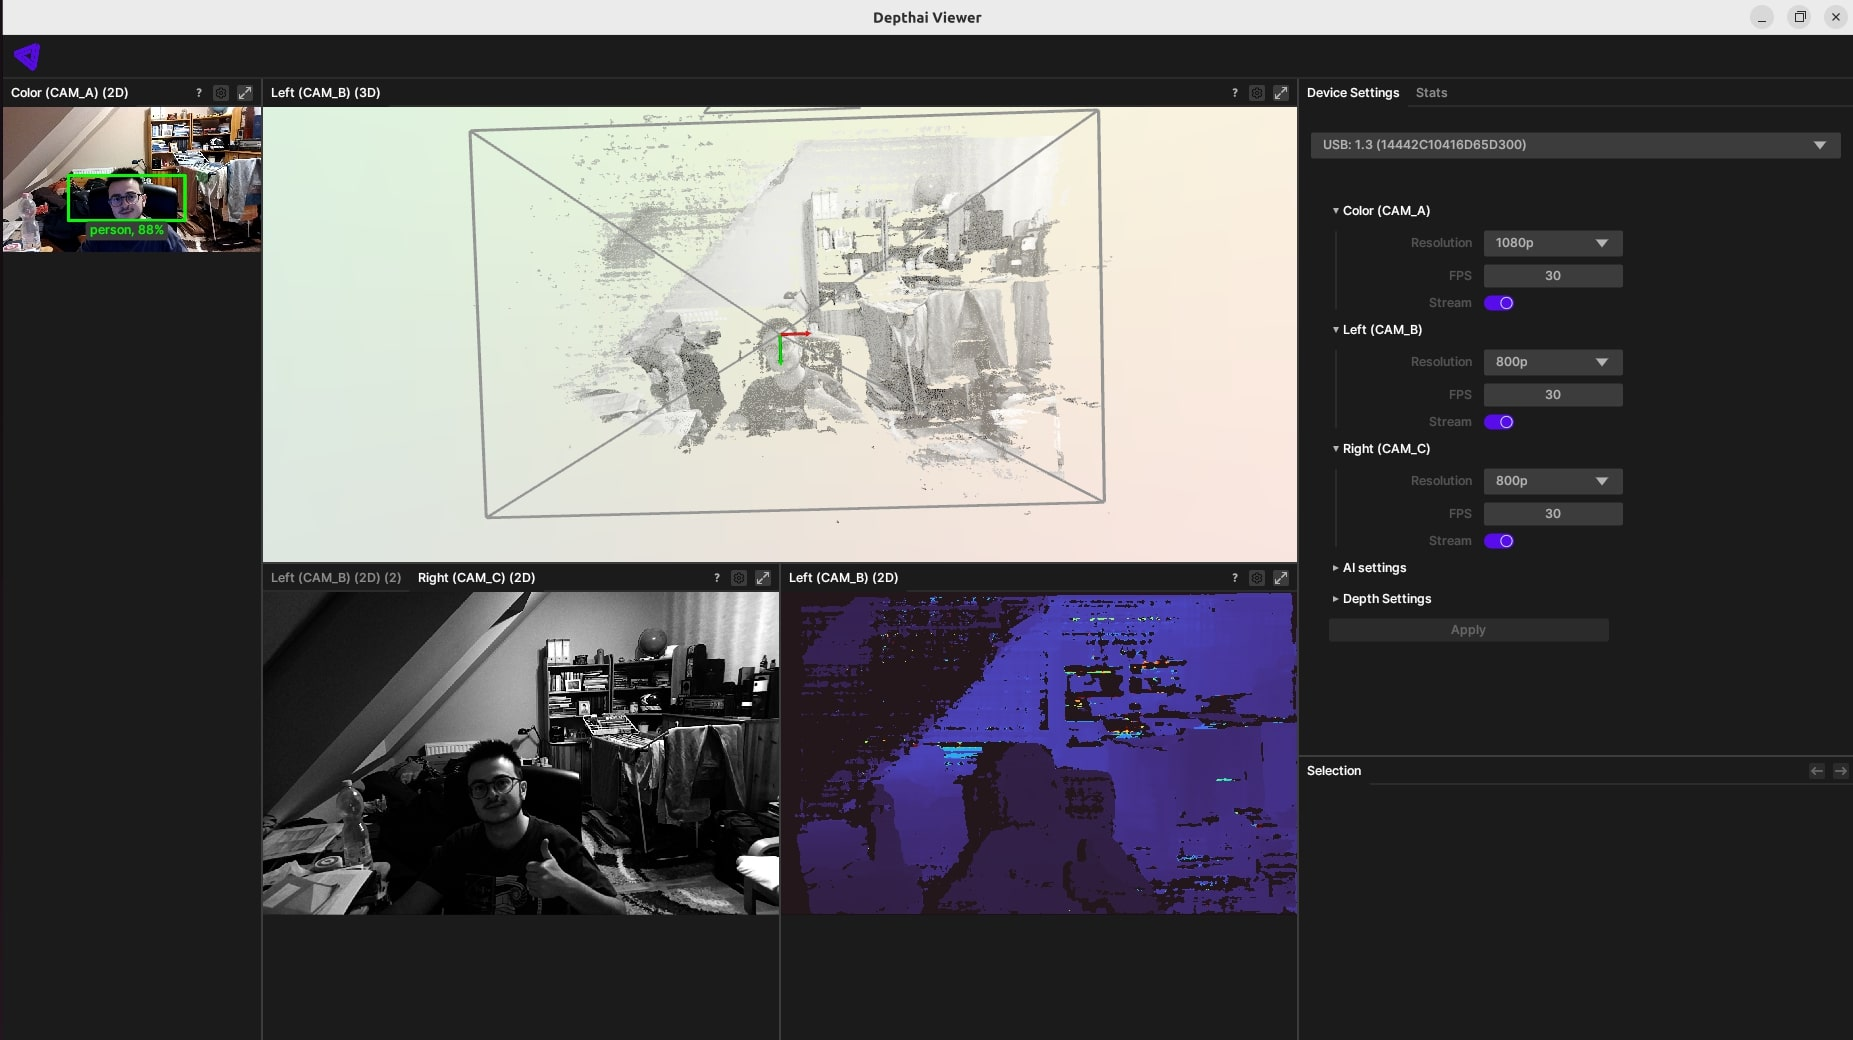
\includegraphics[width=150mm, keepaspectratio]{figures_jpg/depthai_viewer.jpg}
	\caption{DepthAI Viewer with person detection}
	\label{fig:DAI_person_detection}
\end{figure}

\begin{figure}[htbp]
	\centering
	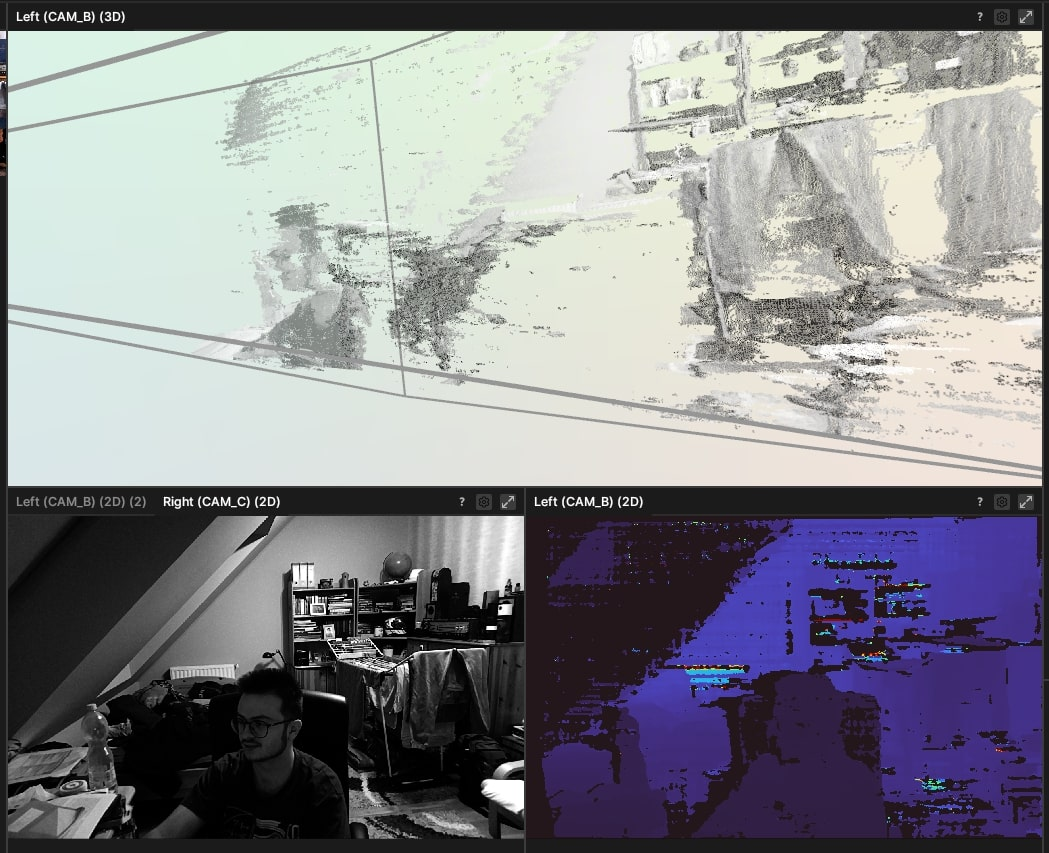
\includegraphics[width=150mm, keepaspectratio]{figures_jpg/depthai_viewer_3d.jpg}
	\caption{DepthAI Viewer's 3D reconstruction}
	\label{fig:DAI_3d}
\end{figure}
\FloatBarrier

This initial exploration served as a foundational step in understanding the camera's capabilities and paved the way for further experimentation and development in subsequent tasks.


\section{Experimenting with Spectacular AI} \label{experiments_spai}

The next step involved experimenting with examples from the Spectacular AI SDK to evaluate its capabilities for mapping and low-latency person detection. Initially, the provided Python scripts raised warnings and failed to execute properly:

\FloatBarrier
\begin{lstlisting}[language=bash,frame=single,float=h]
SpectacularAI WARN: Dropping frames!
SpectacularAI WARN: VIO may be running too slow, data is being input too fast, or IMU samples are missing / time-offset from frames. (buffer size 10)
\end{lstlisting}
\FloatBarrier

After research, I discovered that these issues were due to outdated firmware on the camera, an issue that was challenging to identify due to sparse documentation. To resolve this, I cloned Luxonis' \verb|depthai-python| repository\footnote{\url{https://github.com/luxonis/depthai-python}} and ran the IMU firmware update script\footnote{\url{https://github.com/luxonis/depthai-python/blob/main/examples/IMU/imu_firmware_update.py}}. Following the successful firmware update, I was able to run the examples without issues.

The simplest example visualized the camera’s movement by extracting IMU data and plotting it using matplotlib. As shown in Figure~\ref{fig:IMU_visu}, I was able to "draw" a heart in the air. The curves are slightly uneven due to minor hand movements.

\begin{figure}[htbp]
	\centering
	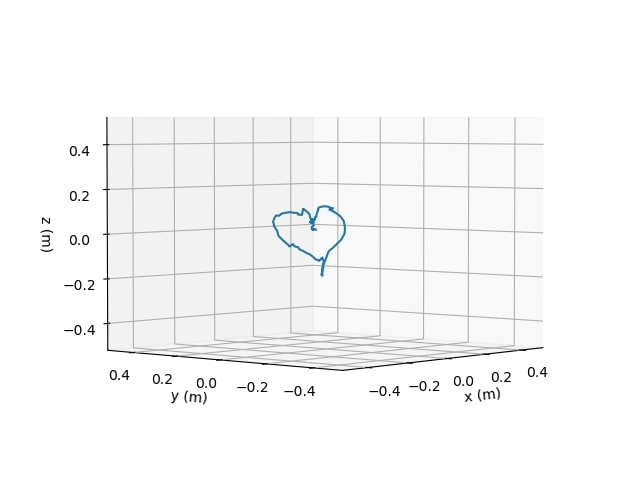
\includegraphics[width=150mm, keepaspectratio]{figures_jpg/spectacular_ai_vio_visu.jpg}
	\caption{IMU visualization with Spectacular AI}
	\label{fig:IMU_visu}
\end{figure}

A more advanced example uses both the camera and the IMU. The device only visualizes movement using IMU data when the camera lens are covered, as shown in Figure~\ref{fig:3d_pen}.

\begin{figure}[htbp]
	\centering
	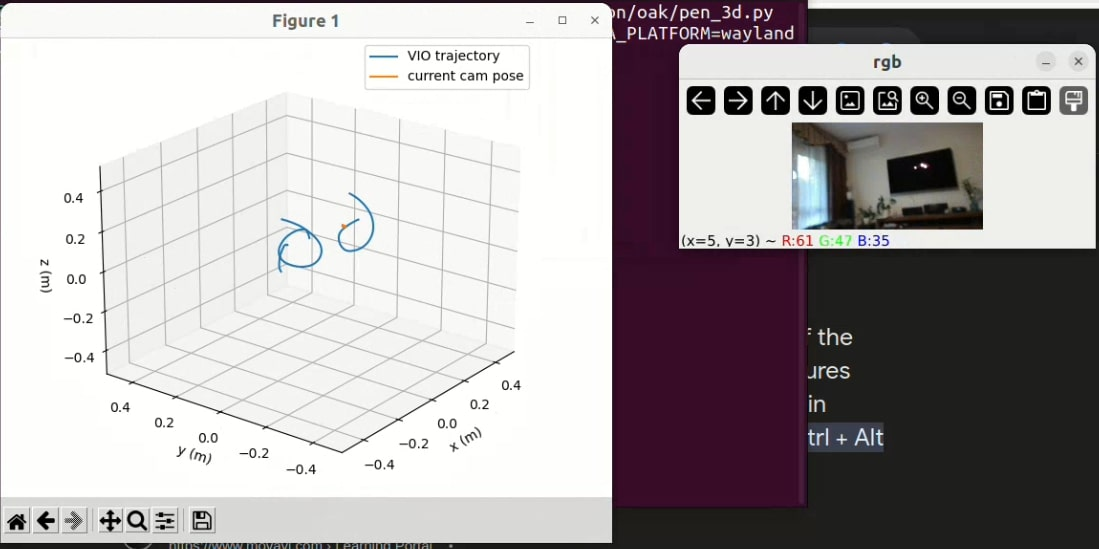
\includegraphics[width=150mm, keepaspectratio]{figures_jpg/3d_pen.jpg}
	\caption{IMU visualization with Spectacular AI}
	\label{fig:3d_pen}
\end{figure}

While these initial examples primarily demonstrated movement visualization, the SDK also includes more sophisticated examples for mapping and object detection. However, these examples raised errors due to issues in the OpenGL-based visualization. To address this, I modified the \verb|OpenGL/contexdata.py| file by commenting out specific lines, as shown below:

\begin{lstlisting}[language=python,frame=single,float=!ht]
def getContext( context = None ):
    """Get the context (if passed, just return)
    context -- the context ID, if None, the current context
    """
    if context is None:
        context = platform.GetCurrentContext()
    # if context == 0:
        # from OpenGL import error
        # raise error.Error(
        # """Attempt to retrieve context when no valid context"""
        # )
    return context
\end{lstlisting}
\FloatBarrier

This adjustment allowed me to run various mapping examples, including point cloud mapping (Figure~\ref{fig:SPAI_mapping}), real-time AR mapping with mesh (Figure~\ref{fig:SPAI_mesh_mapping}), real-time AR mapping with point cloud (Figure~\ref{fig:SPAI_point_cloud_mapping}), and ROS2-integrated mapping (Figure~\ref{fig:SPAI_ros_mapping}).

\begin{figure}[htbp]
	\centering
	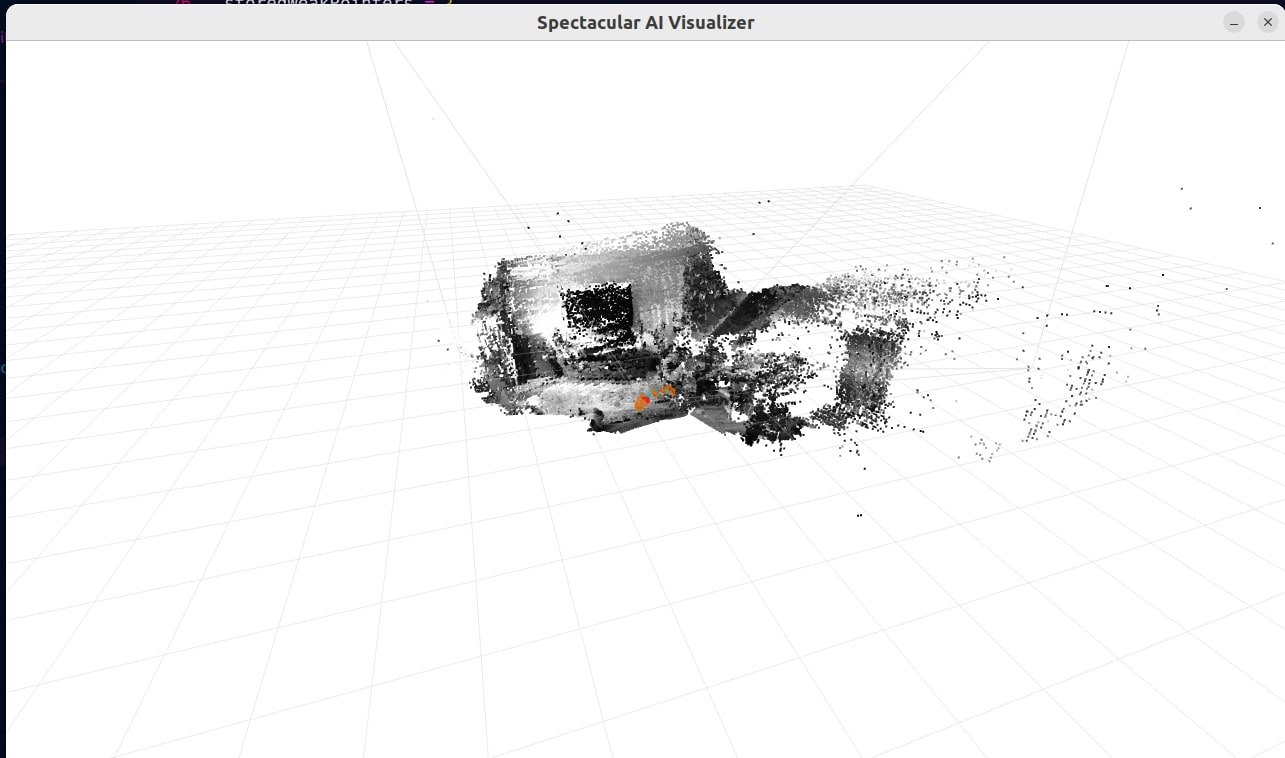
\includegraphics[width=150mm, keepaspectratio]{figures_jpg/spectacular_ai_mapping_visu.jpg}
	\caption{Mapping with Spectacular AI}
	\label{fig:SPAI_mapping}
\end{figure}

\begin{figure}[htbp]
	\centering
	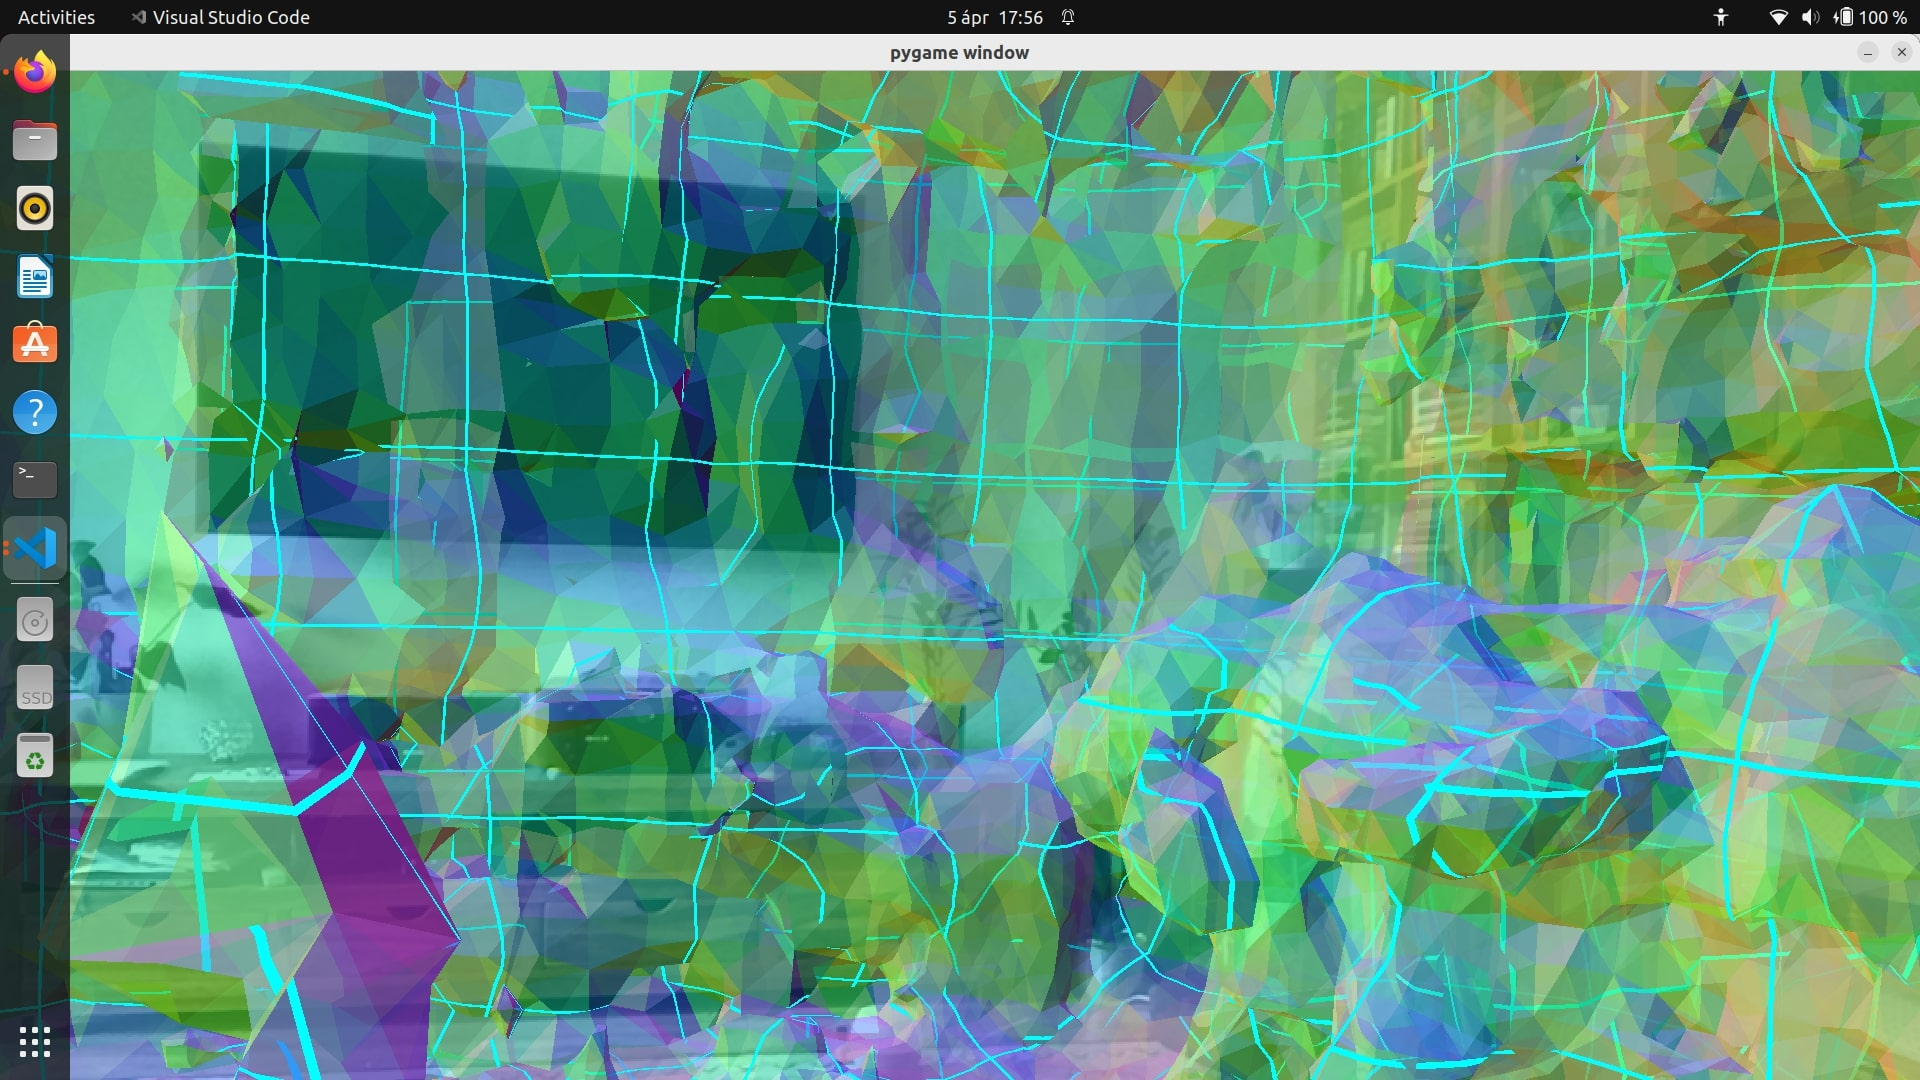
\includegraphics[width=67mm, keepaspectratio]{figures_jpg/spectacular_ai_mapping_ar_mesh1.jpg}\hspace{1cm}
	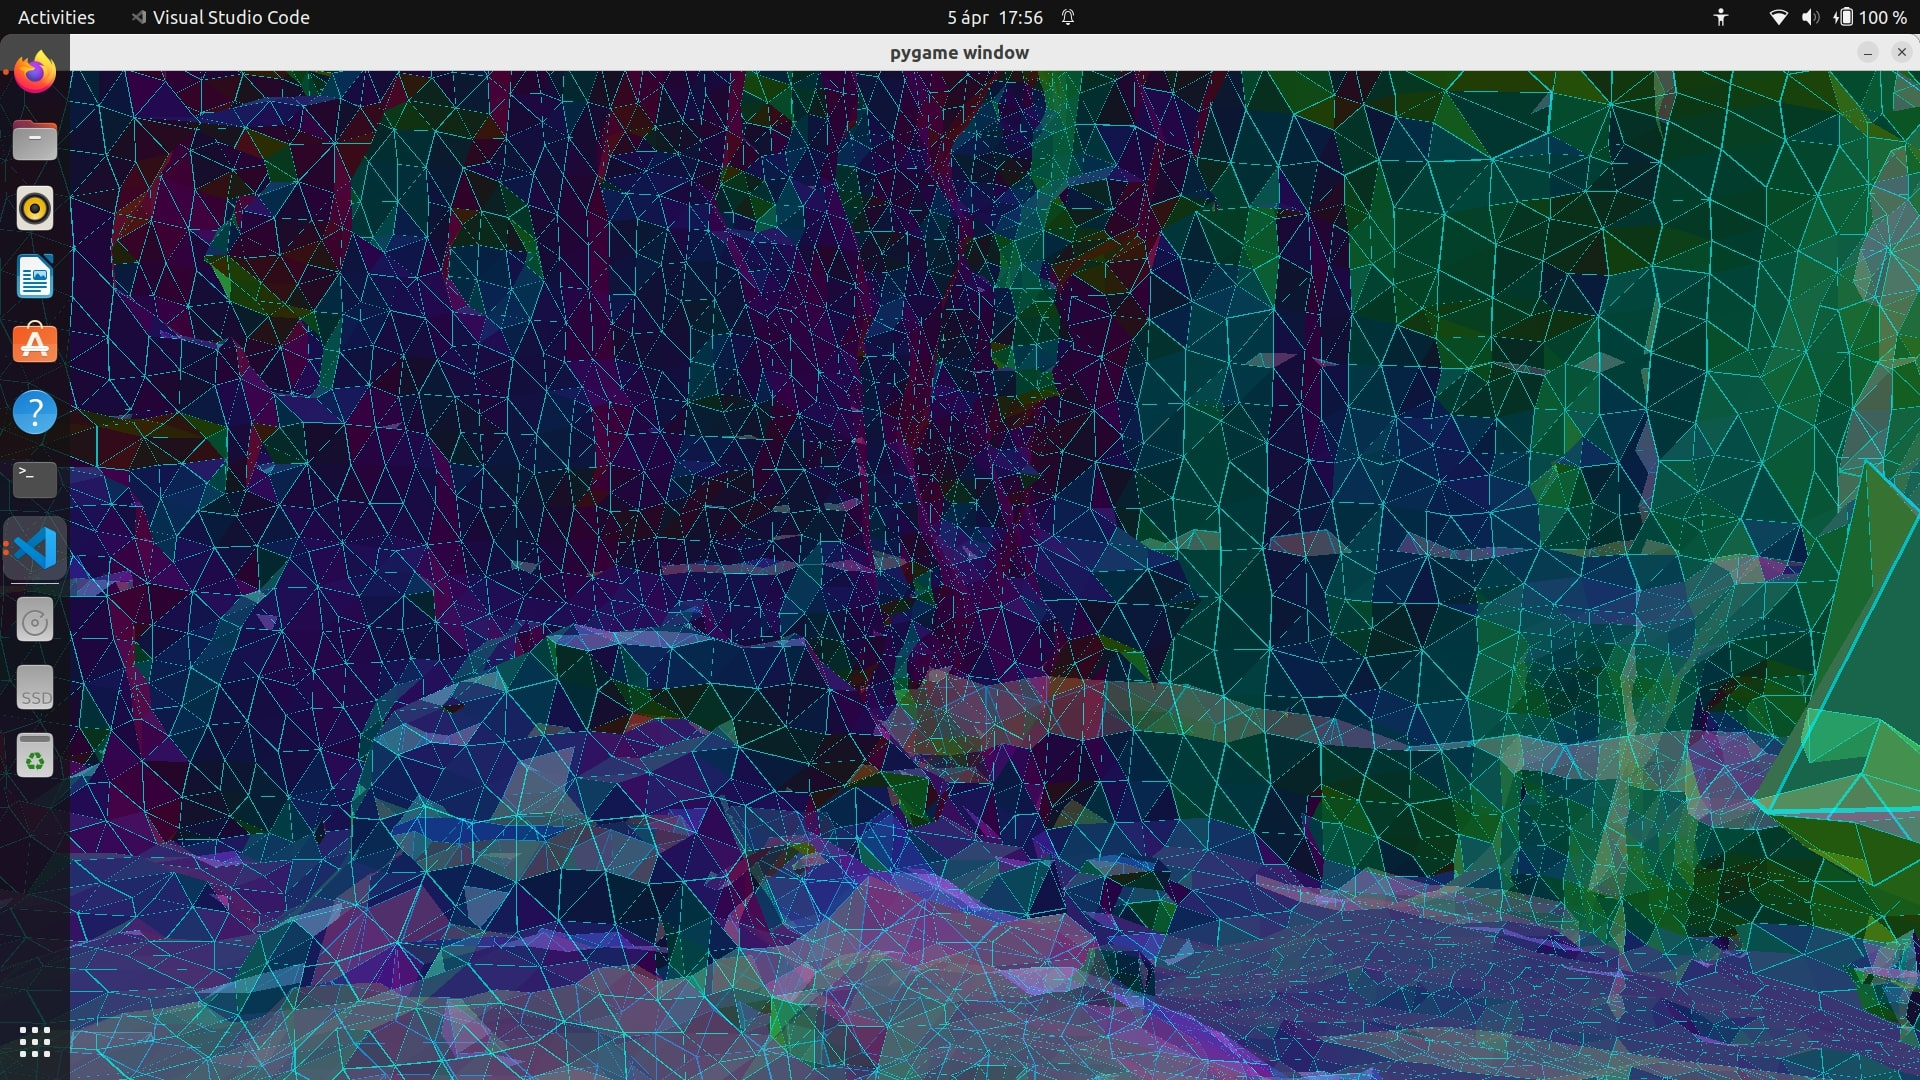
\includegraphics[width=67mm, keepaspectratio]{figures_jpg/spectacular_ai_mapping_ar_mesh2.jpg}\\\vspace{5mm}
	\caption{AR mesh mapping with Spectacular AI}
    \label{fig:SPAI_mesh_mapping}
\end{figure}

\begin{figure}[htbp]
	\centering
	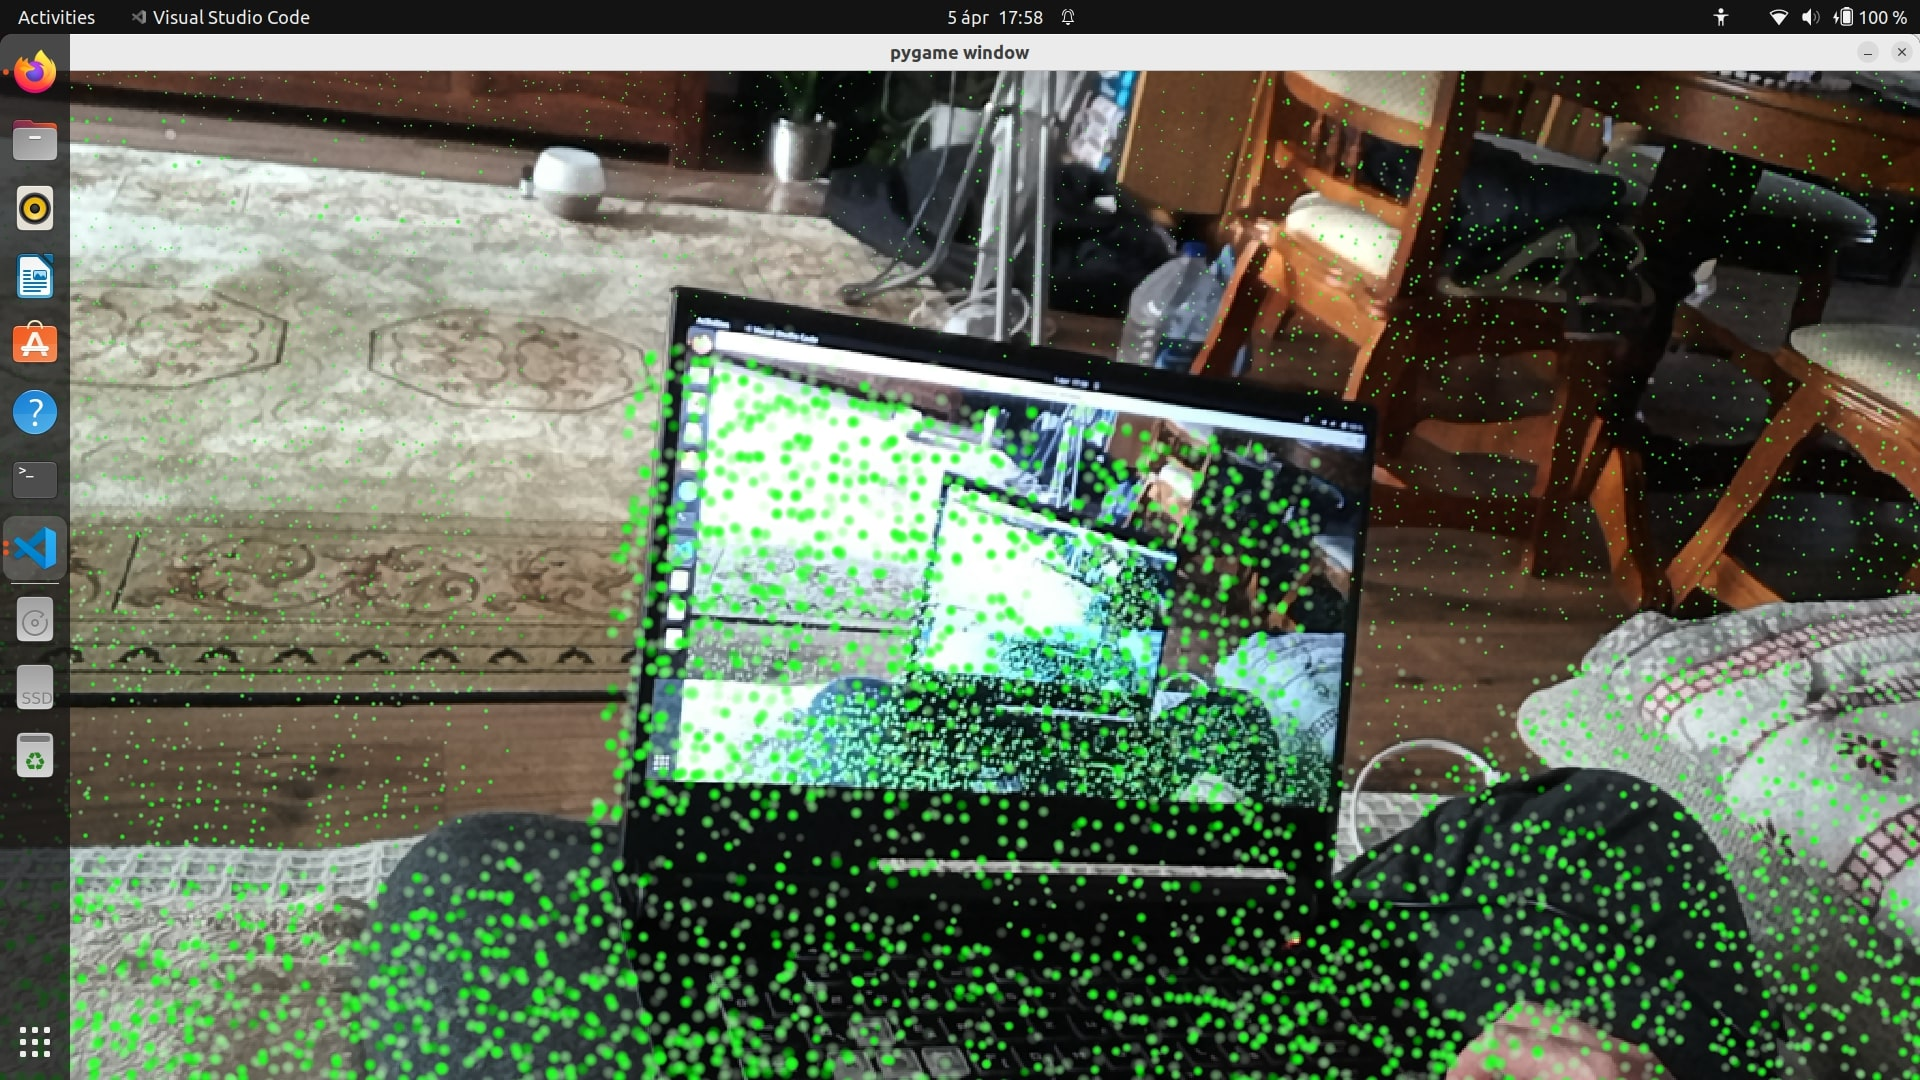
\includegraphics[width=67mm, keepaspectratio]{figures_jpg/spectacular_ai_mapping_ar_pc1.jpg}\hspace{1cm}
	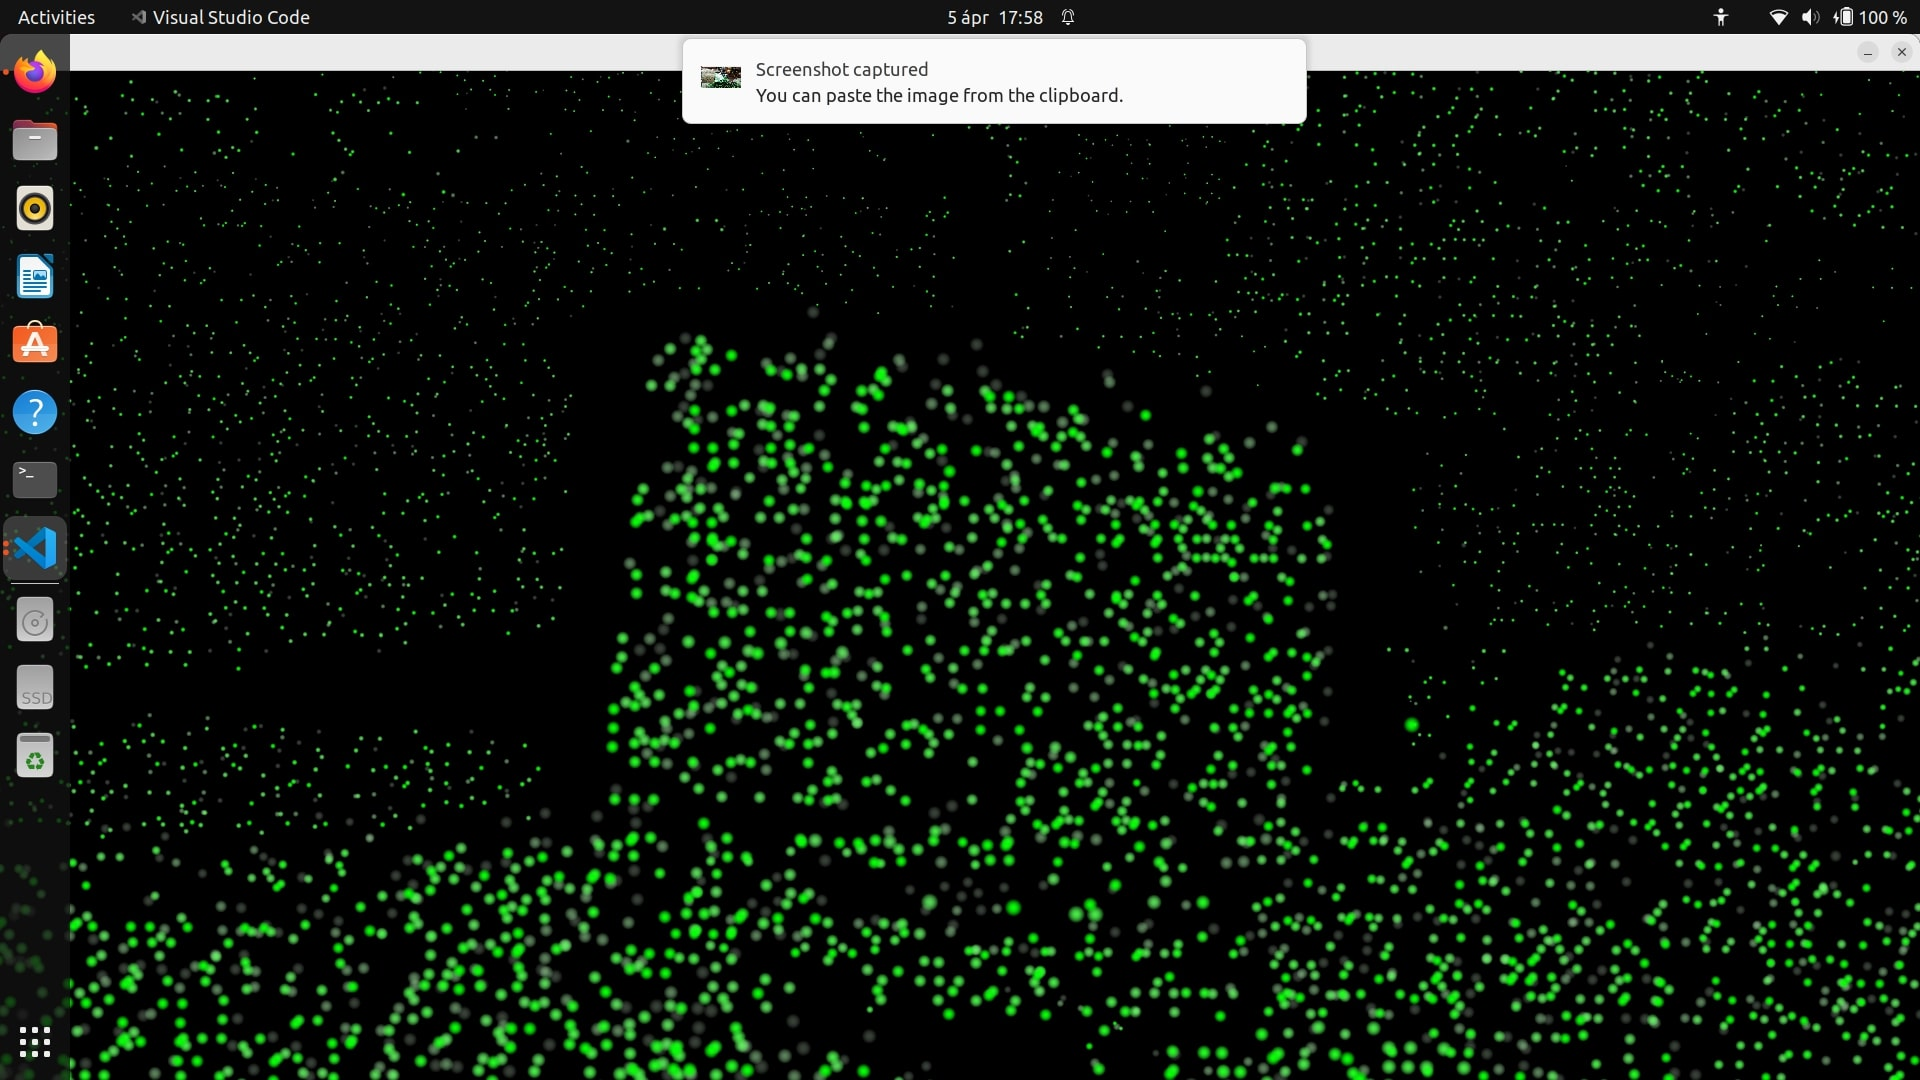
\includegraphics[width=67mm, keepaspectratio]{figures_jpg/spectacular_ai_mapping_ar_pc2.jpg}\\\vspace{5mm}
	\caption{AR point cloud mapping with Spectacular AI}
    \label{fig:SPAI_point_cloud_mapping}
\end{figure}

\begin{figure}[htbp]
	\centering
	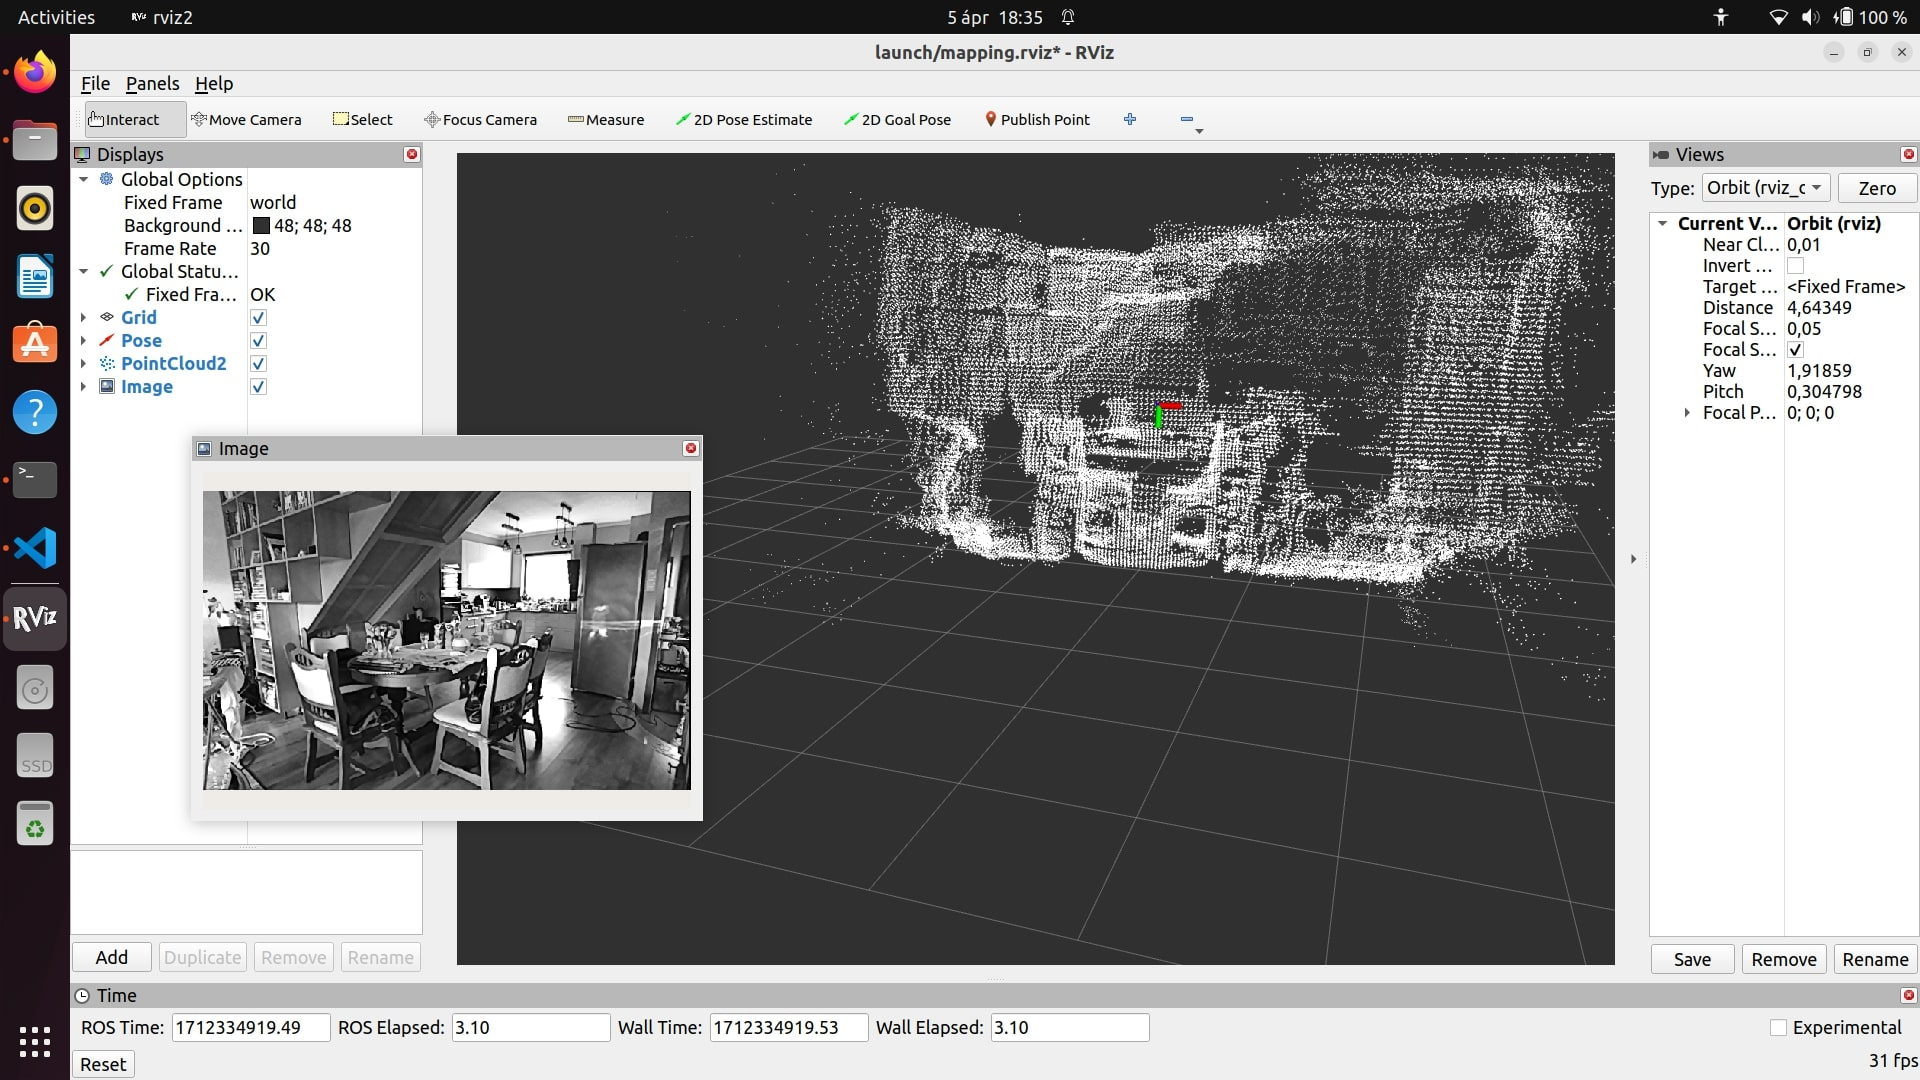
\includegraphics[width=150mm, keepaspectratio]{figures_jpg/spectacular_ai_mapping_ros2.jpg}
	\caption{ROS2 mapping with Spectacular AI}
	\label{fig:SPAI_ros_mapping}
\end{figure}

Through testing, I found that the Spectacular AI SDK worked efficiently with the OAK camera, with no major latency issues, confirming its suitability for real-time applications.

The final example I explored highlights one of the most impressive capabilities of the OAK-D camera, which is powered by an Intel Movidius Myriad X VPU\footnote{\url{https://www.intel.com/content/www/us/en/products/sku/204770/intel-movidius-myriad-x-vision-processing-unit-0gb/specifications.html}}. This VPU enables the camera to run neural networks directly on the device, allowing real-time object detection and position estimation. By modifying a single list in the example code, I customized the detection to identify potted plants, as shown in Figure~\ref{fig:SPAI_depthai}. Despite some challenges with lighting, the detections were accurate, with precise distance calculations matching my manual measurements. This feature is extremely useful for our purposes, as it allows object detection in 3D space alongside camera pose tracking, enabling accurate estimation of object locations in the environment.

\begin{figure}[htbp]
	\centering
	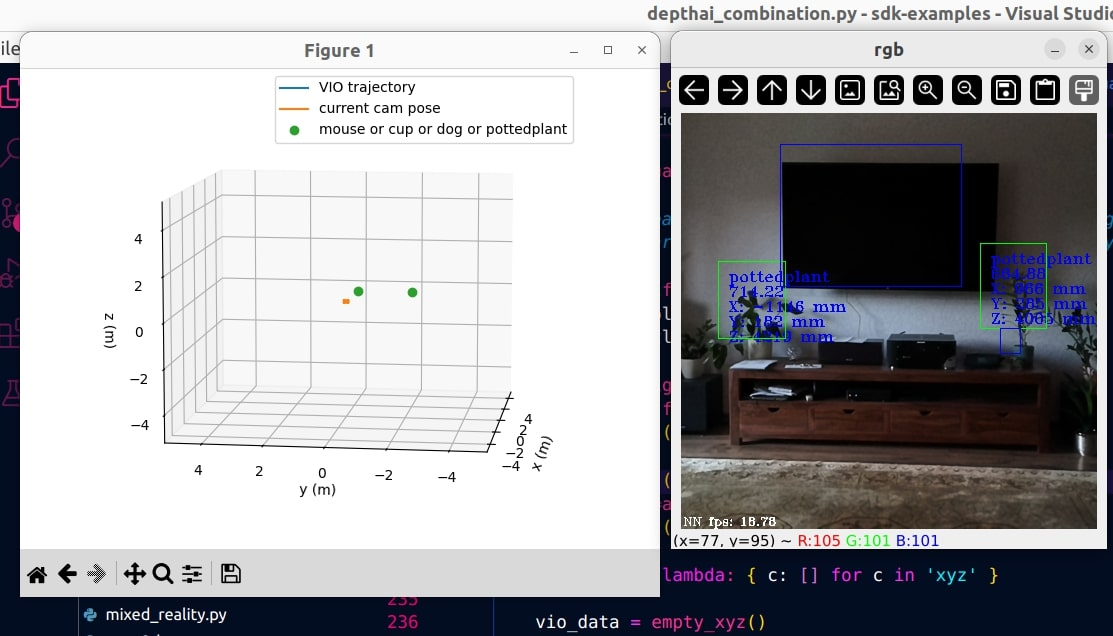
\includegraphics[width=150mm, keepaspectratio]{figures_jpg/spectacular_ai_depthai_combination.jpg}
	\caption{Spectacular AI's object detection and position calculation}
	\label{fig:SPAI_depthai}
\end{figure}


\section{Experimenting with a Custom Person Detector}

One of our objectives was to detect people using the robot's camera and enable the robot to follow or avoid them while mapping. We initially tested Spectacular AI’s example detection model on the robot’s camera, but quickly realized that its default placement restricted the field of view (FOV). Due to the platform above the robot, the camera’s FOV was so limited that, at a distance of 2–3 meters, only a person’s legs were visible, which rendered the detection ineffective.

To resolve this, we repositioned the camera at the front edge of the platform, temporarily mounting it with plasticine, which significantly improved the FOV. This adjustment allowed clearer detection, as shown in Figure \ref{fig:person_detection_camera_at_front_nokia}, where my advisor is detected (the other detected individual is a person on a poster).

After adjusting the FOV and testing the example detection script, I developed a custom script based on the example, designed to detect people and publish their locations in world coordinates on a ROS topic (code available in Appendix \ref{custom_person_detector}). However, both the base example and my custom person detector frequently froze after several detections, with an error related to the IMU buffer size. This issue occurred because the IMU data rate was too high, and the \verb|SpatialLocationCalculator| node’s buffer size was inadequate and inflexible. This buffer could not be extended or flushed due to its fixed nature within the node.

In conclusion, while the repositioned camera improved FOV, the camera's current limitations in buffer handling prevented us from implementing a stable person detection system.

\begin{figure}[htbp]
    \centering
    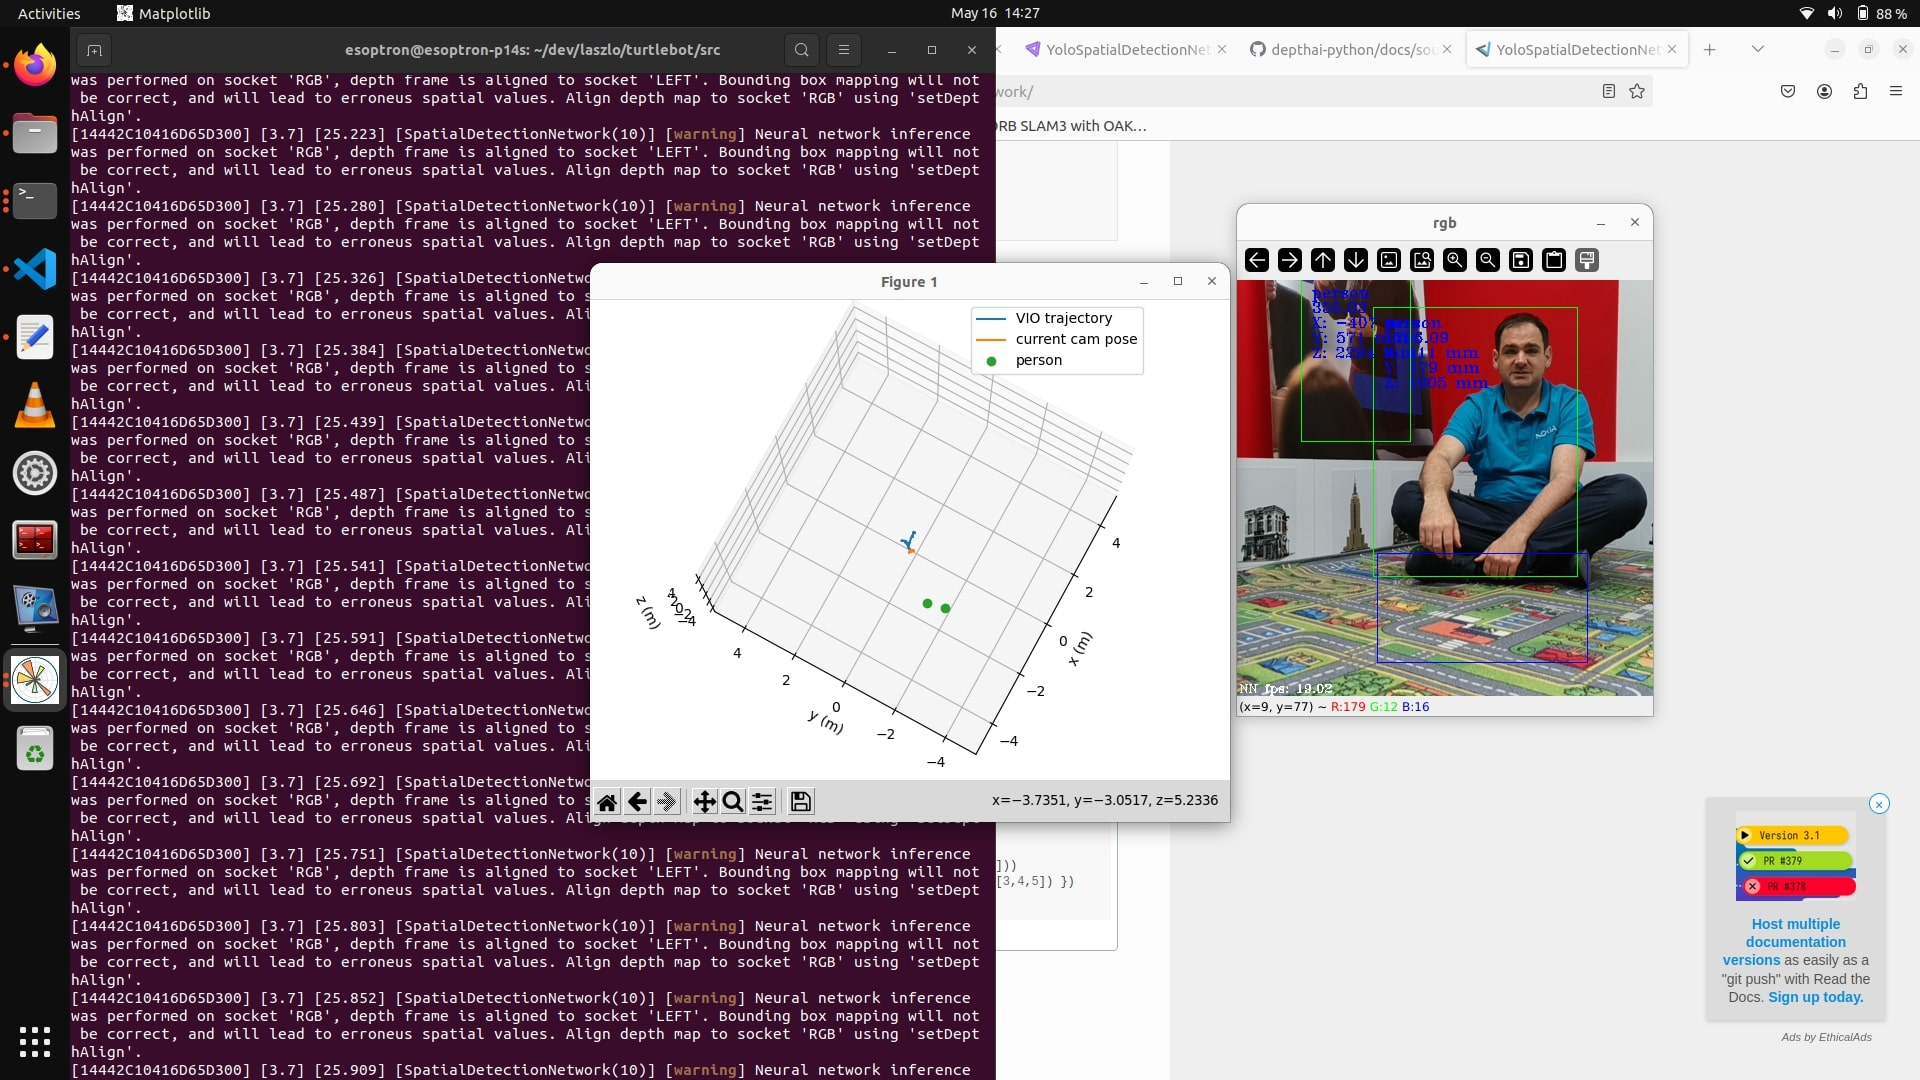
\includegraphics[width=150mm, keepaspectratio]{figures_jpg/person_detection_camera_at_front_nokia.jpg}
    \caption{Person detection with the camera at front at Nokia Bell Labs}
    \label{fig:person_detection_camera_at_front_nokia}
\end{figure}
